\documentclass[handout]{beamer}
\usepackage{animate}
\graphicspath{{../figure}}
\usepackage{listings}
\sffamily
\setbeamertemplate{itemize items}[circle]
\usepackage{xcolor}\usepackage{tcolorbox}
\usepackage{mathtools}

\definecolor{codegreen}{rgb}{0,0.6,0}
\definecolor{codegray}{rgb}{0.5,0.5,0.5}
\definecolor{codepurple}{rgb}{0.58,0,0.82}
\definecolor{backcolour}{rgb}{0.95,0.95,0.92}
\definecolor{lightgray}{rgb}{0.95,0.95,0.95}

\lstset{
    commentstyle=\color{codegreen},
    numberstyle=\tiny\color{codegray},
    keywordstyle=\color{codepurple},  
    language=Matlab,
    basicstyle=\scriptsize,
    backgroundcolor=\color{lightgray},
    tabsize=2
}

\title{Path planning locale per robot mobili basato su switching tra potenziali artificiali}
\author{Flavio Maiorana}
\date{}

\begin{document}

\frame{\maketitle}

%30 secondi
\begin{frame}{Definizione del Problema}
\framesubtitle{Path planning locale}
Guidare il robot mobile dalla sua \textbf{posizione iniziale} ad un \textbf{punto di goal}, evitando gli \textbf{ostacoli} non noti a priori
\begin{figure}
\centering
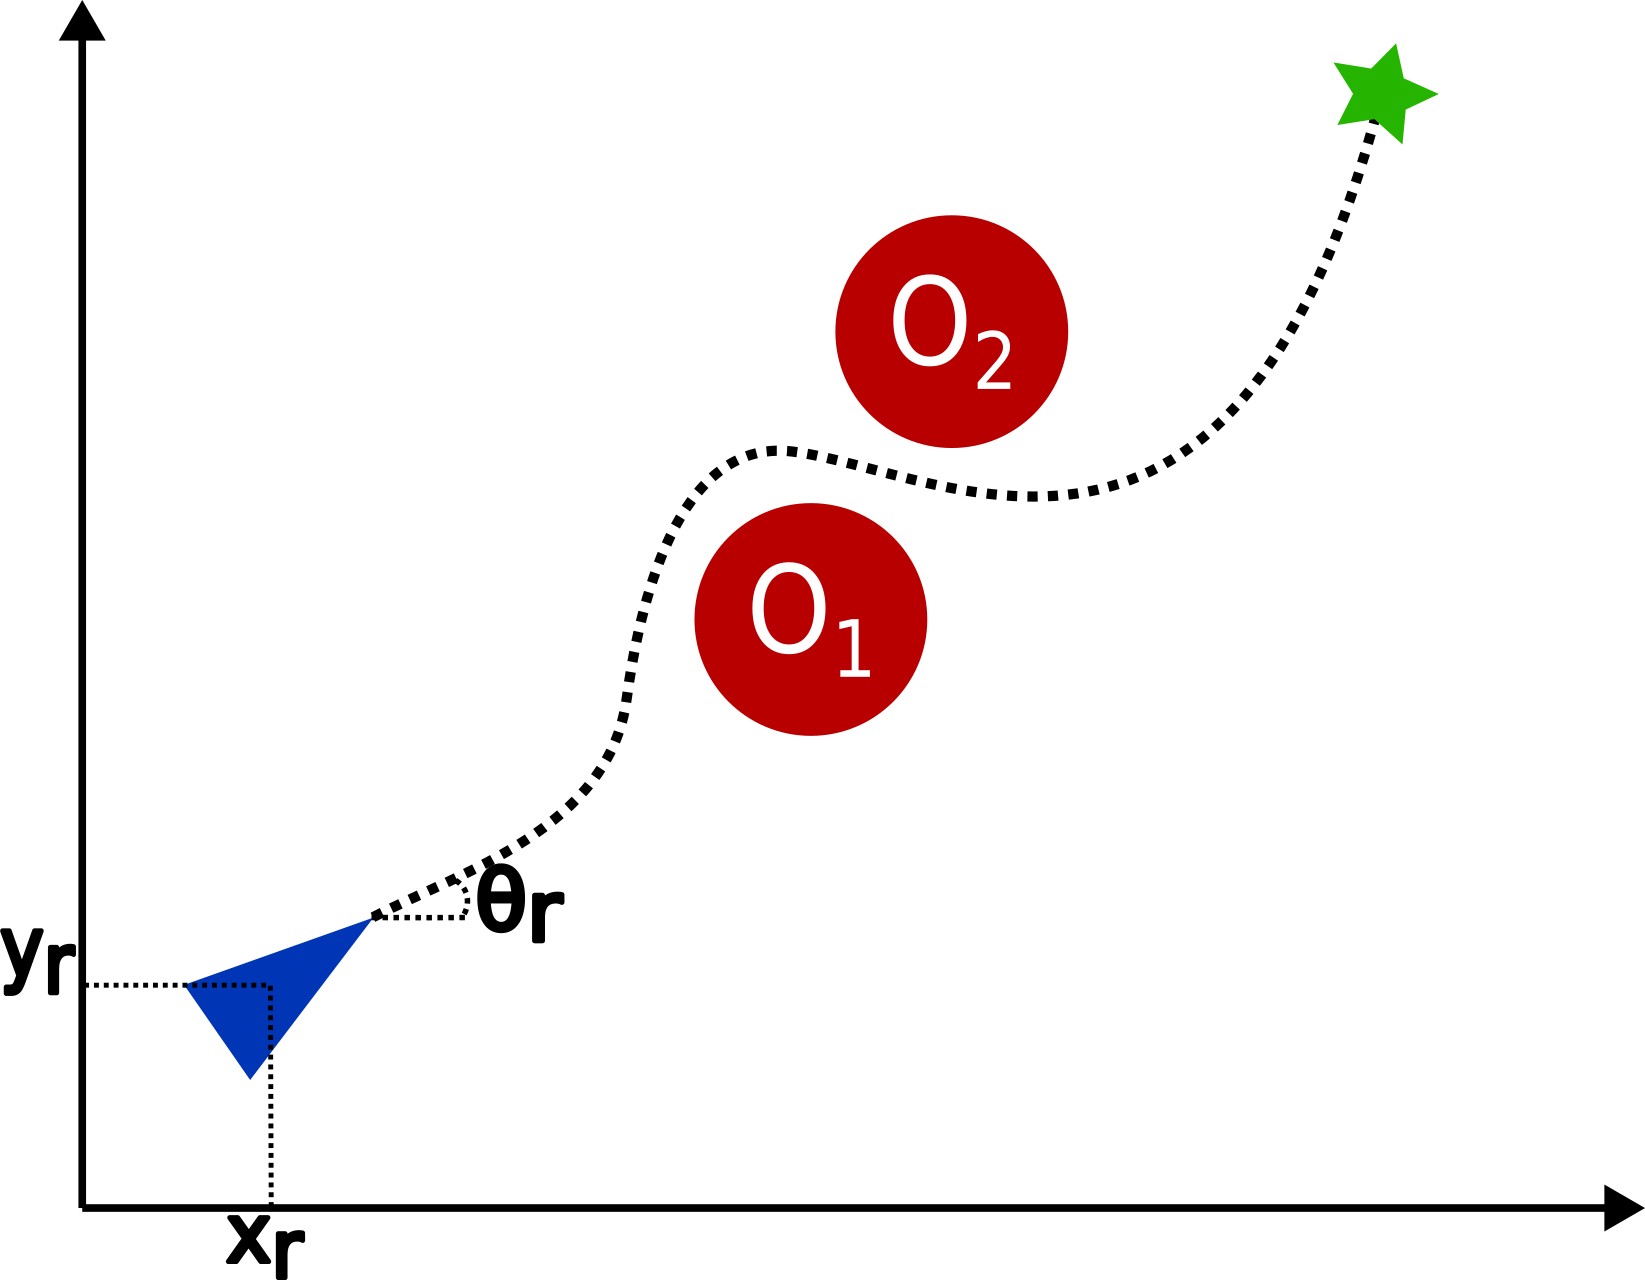
\includegraphics[scale=0.45]{pathplanning.png}
\end{figure}
\end{frame}

%30 secondi
\begin{frame}{Potenziali artificiali}
\framesubtitle{Metodo classico}
\begin{columns}

\column{0.5\textwidth}
	\centering
	{\small Potenziale attrattivo $U_a$}
	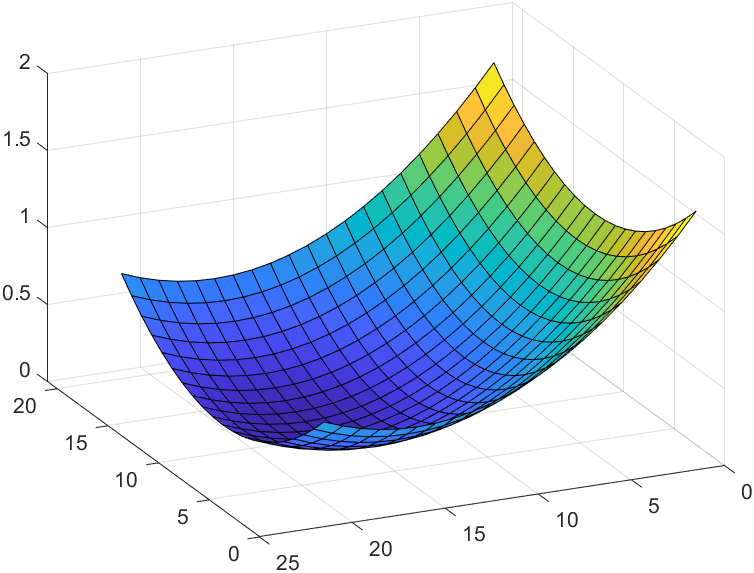
\includegraphics[scale=0.28]{potA.png} \\
	$\downarrow$\\
	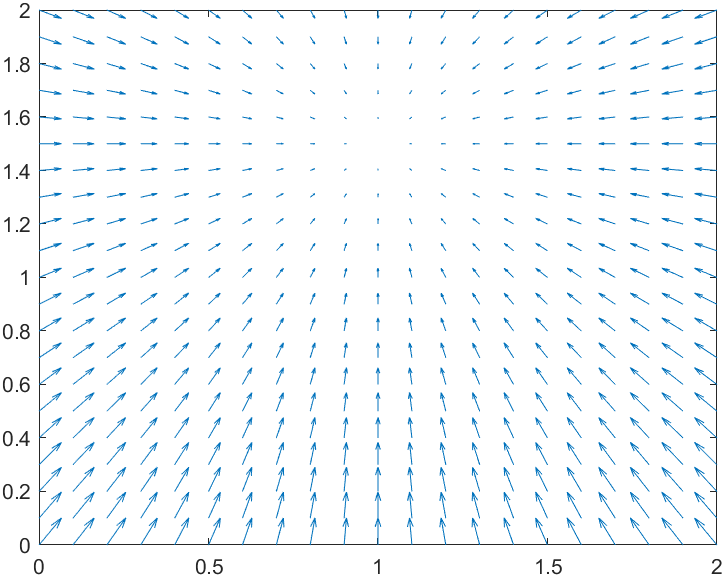
\includegraphics[scale=0.28]{antigradA.png} \\
	$-\nabla U_a$

\column{0.5\textwidth}
	\centering
	{\small Potenziale repulsivo $U_r$}
	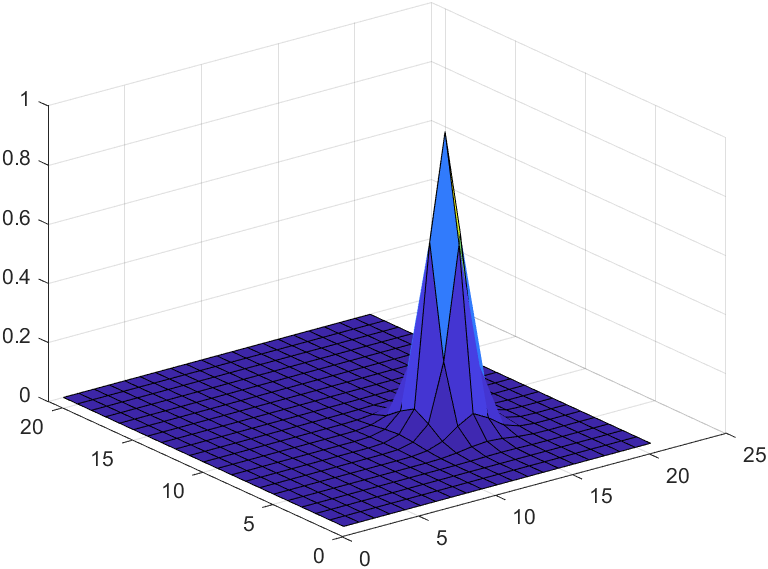
\includegraphics[scale=0.28]{potR.png} \\
	$\downarrow$\\
	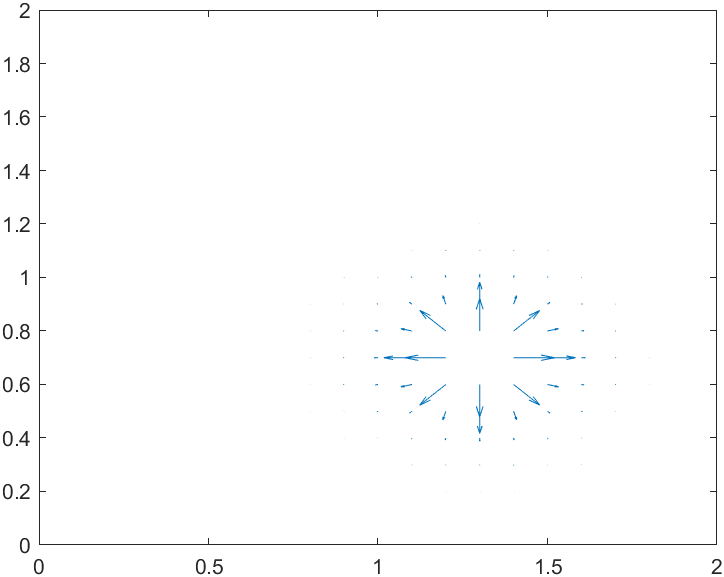
\includegraphics[scale=0.28]{antigradR.png} \\
	$-\nabla U_r$
\end{columns}
\end{frame}

%30 secondi
\begin{frame}{Potenziali artificiali}
\framesubtitle{Metodo classico}

\vspace{5mm}
\begin{columns}
\column{0.45\textwidth}
\centering
\includegraphics[width=\textwidth]{minimolocale_ink.png} \\
Potenziale totale \(U_{tot} = U_a + U_r\)
\column{0.1\textwidth}
\centering
$\rightarrow$
\column{0.45\textwidth}
\centering
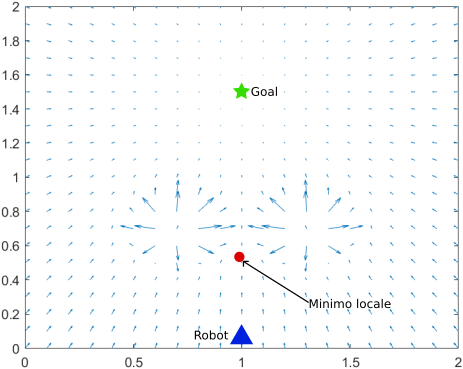
\includegraphics[width=\textwidth]{antigradMinimoLocale.png} \\
Antigradiente $-\nabla U_{tot}$ \\
(Velocità di riferimento)
\end{columns}

\vspace{10mm}

\centering
\begin{tcolorbox}[colframe=red!50!white , center upper]
\textbf{La somma di potenziali causa il rischio di minimo locale}
\end{tcolorbox}
\end{frame}

%30 secondi
\begin{frame}{Potenziali artificiali}
\framesubtitle{Potenziale bypassante}
\begin{itemize}
\item Alternativa al potenziale repulsivo
\item Antigradiente di forma circolare e non radiale
\item Intensità aumenta con avvicinamento all'ostacolo
\end{itemize}
\vspace{5mm}
\begin{columns}
\column{0.45\textwidth}
\centering
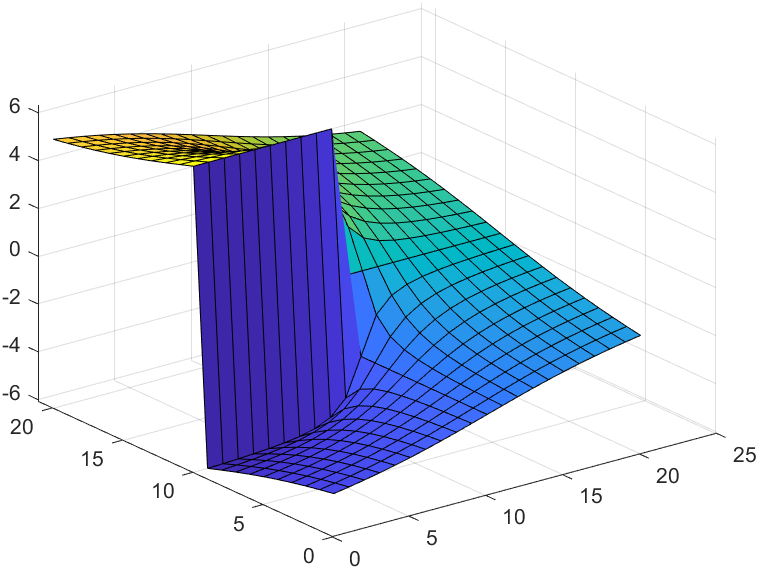
\includegraphics[width=\textwidth]{potB.png} \\
Potenziale totale $U_b$
\column{0.1\textwidth}
\centering
$\rightarrow$
\column{0.45\textwidth}
\centering
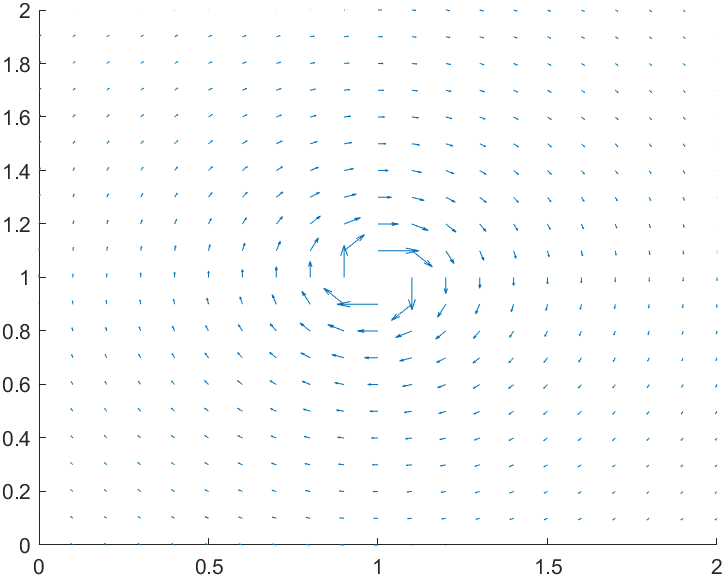
\includegraphics[width=\textwidth]{antigradB.png} \\
Antigradiente $-\nabla U_b$
\end{columns}
\end{frame}

%1 minuto
\begin{frame}{Panoramica sull'algoritmo}	
\centering
Siano $U_a$ e $U_b$ il potenziale attrattivo e bypassante: in ogni $t$ il robot é guidato da un solo potenziale tramite l'antigradiente $-\nabla U$ \\
\vspace*{5mm}
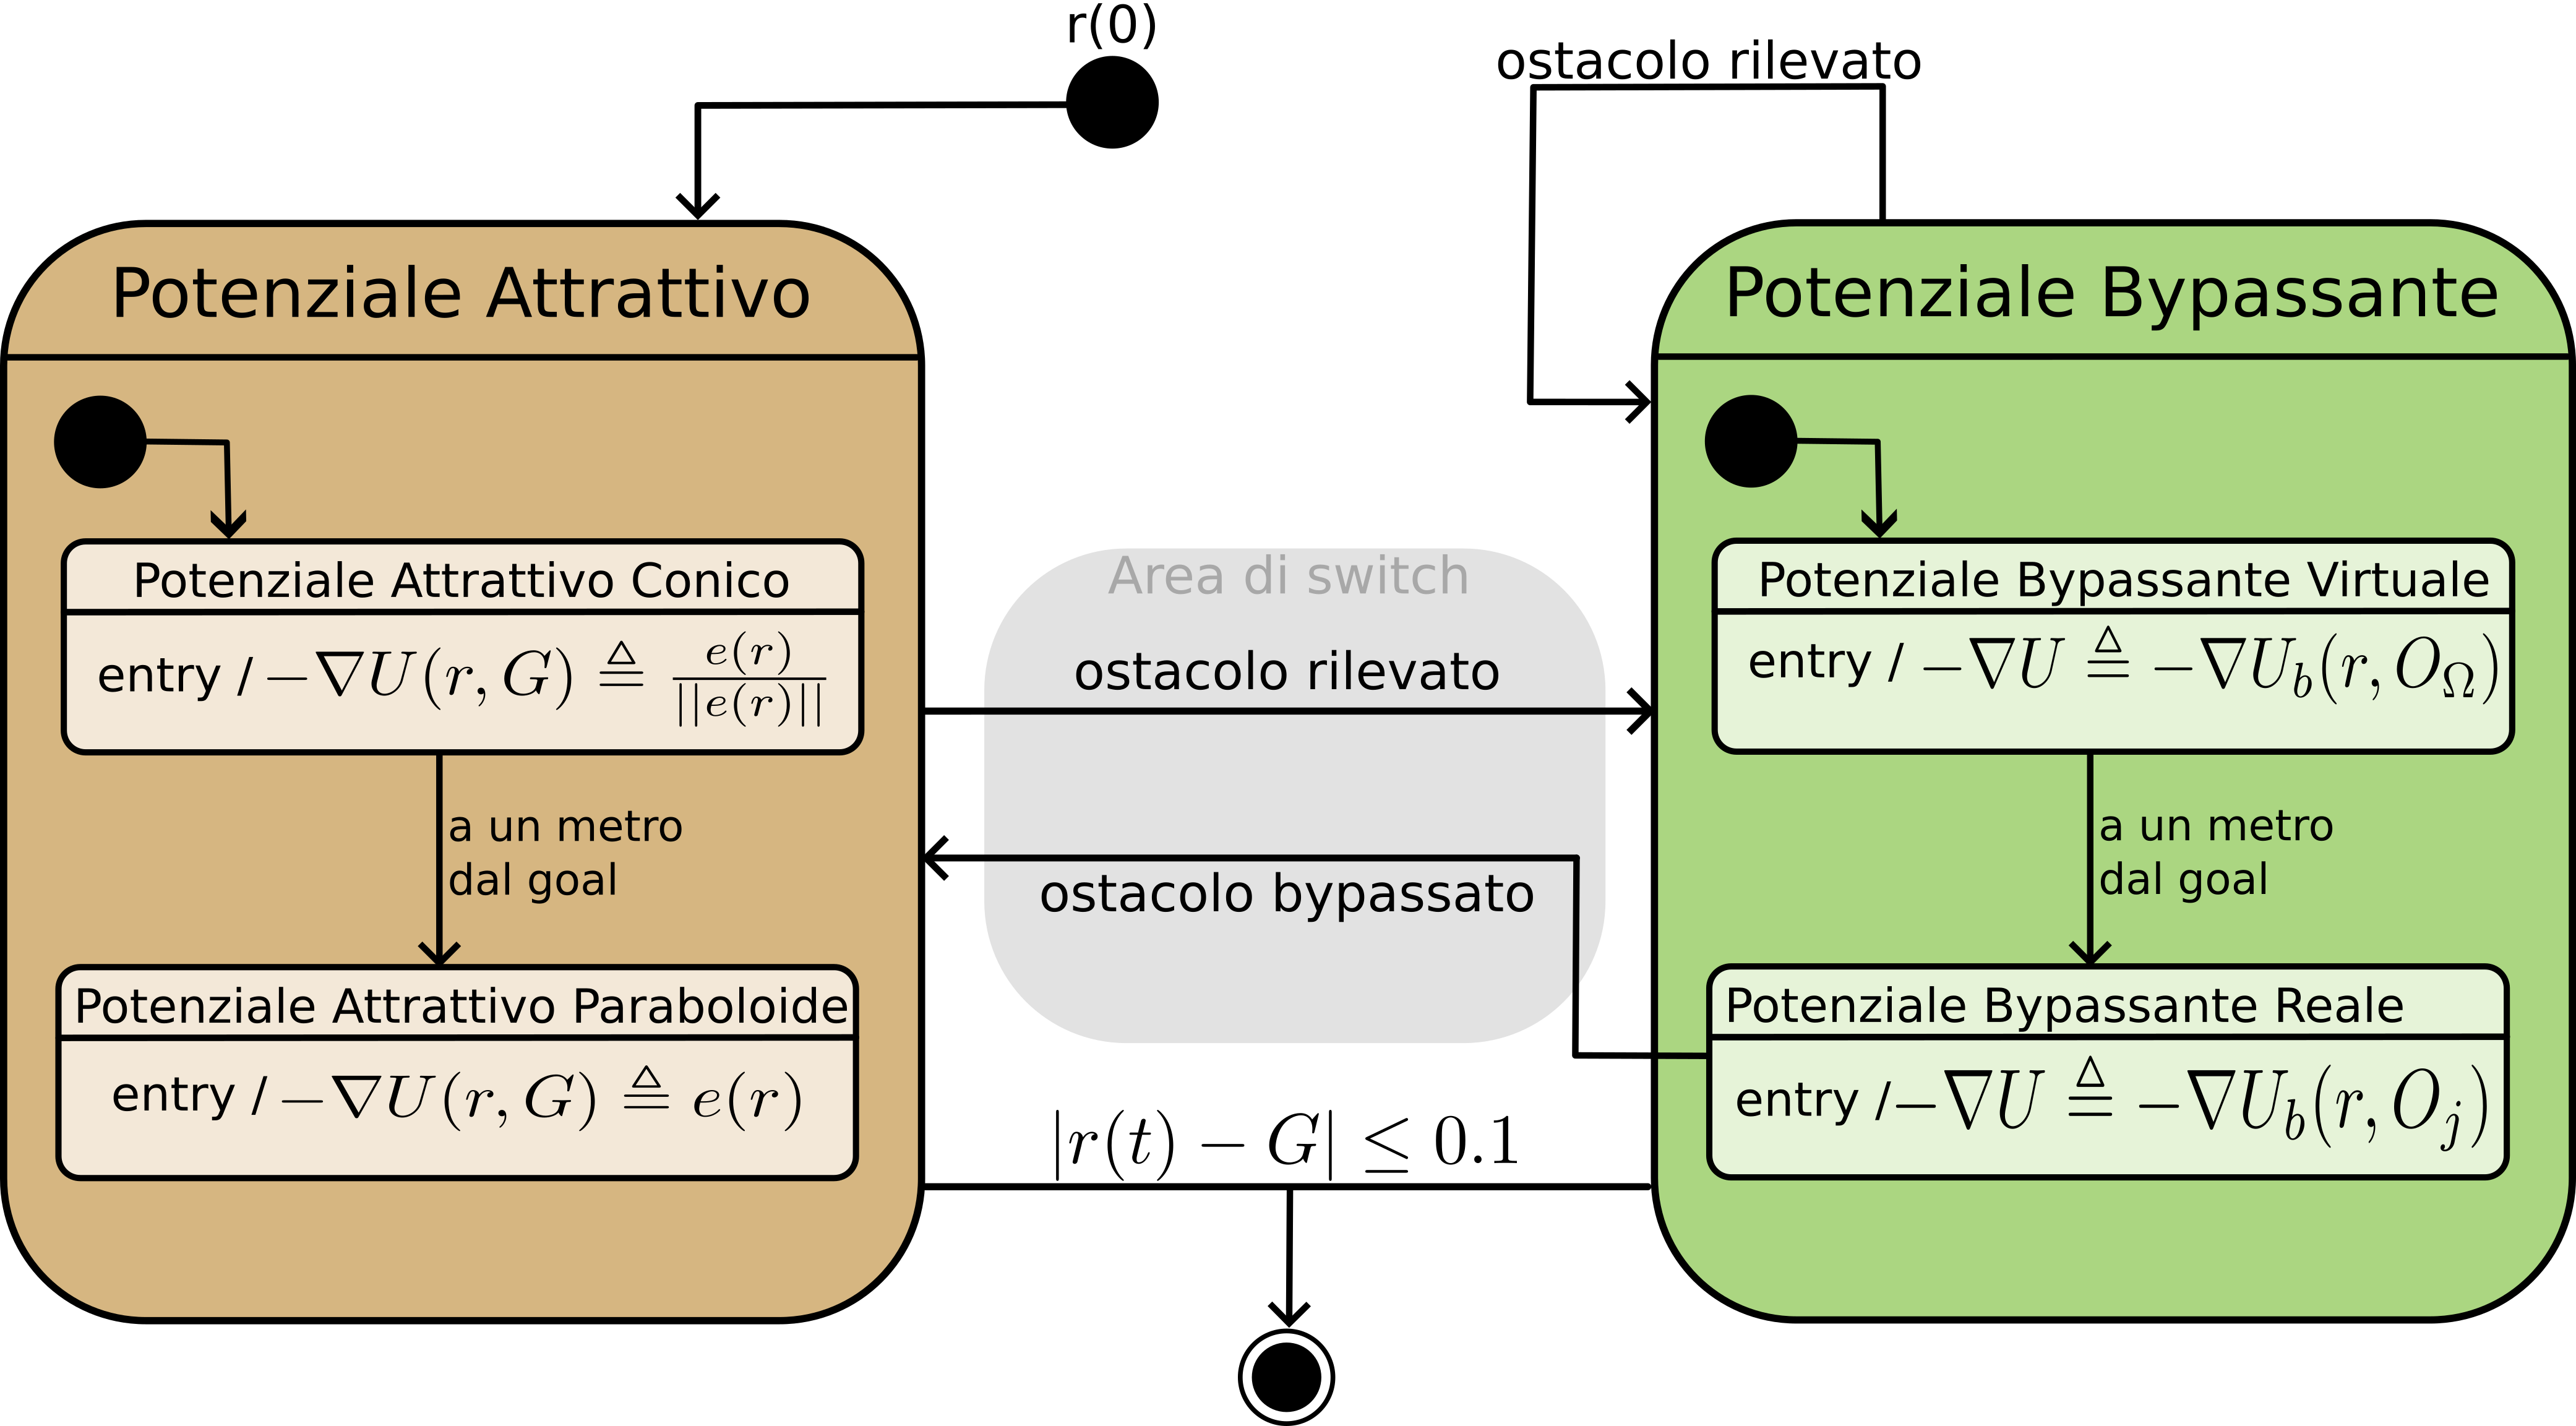
\includegraphics{statechart.png}
\end{frame}

%1 minuto
\begin{frame}[fragile]{Architettura di navigazione}
\begin{columns}
\column{0.5\textwidth}
\centering
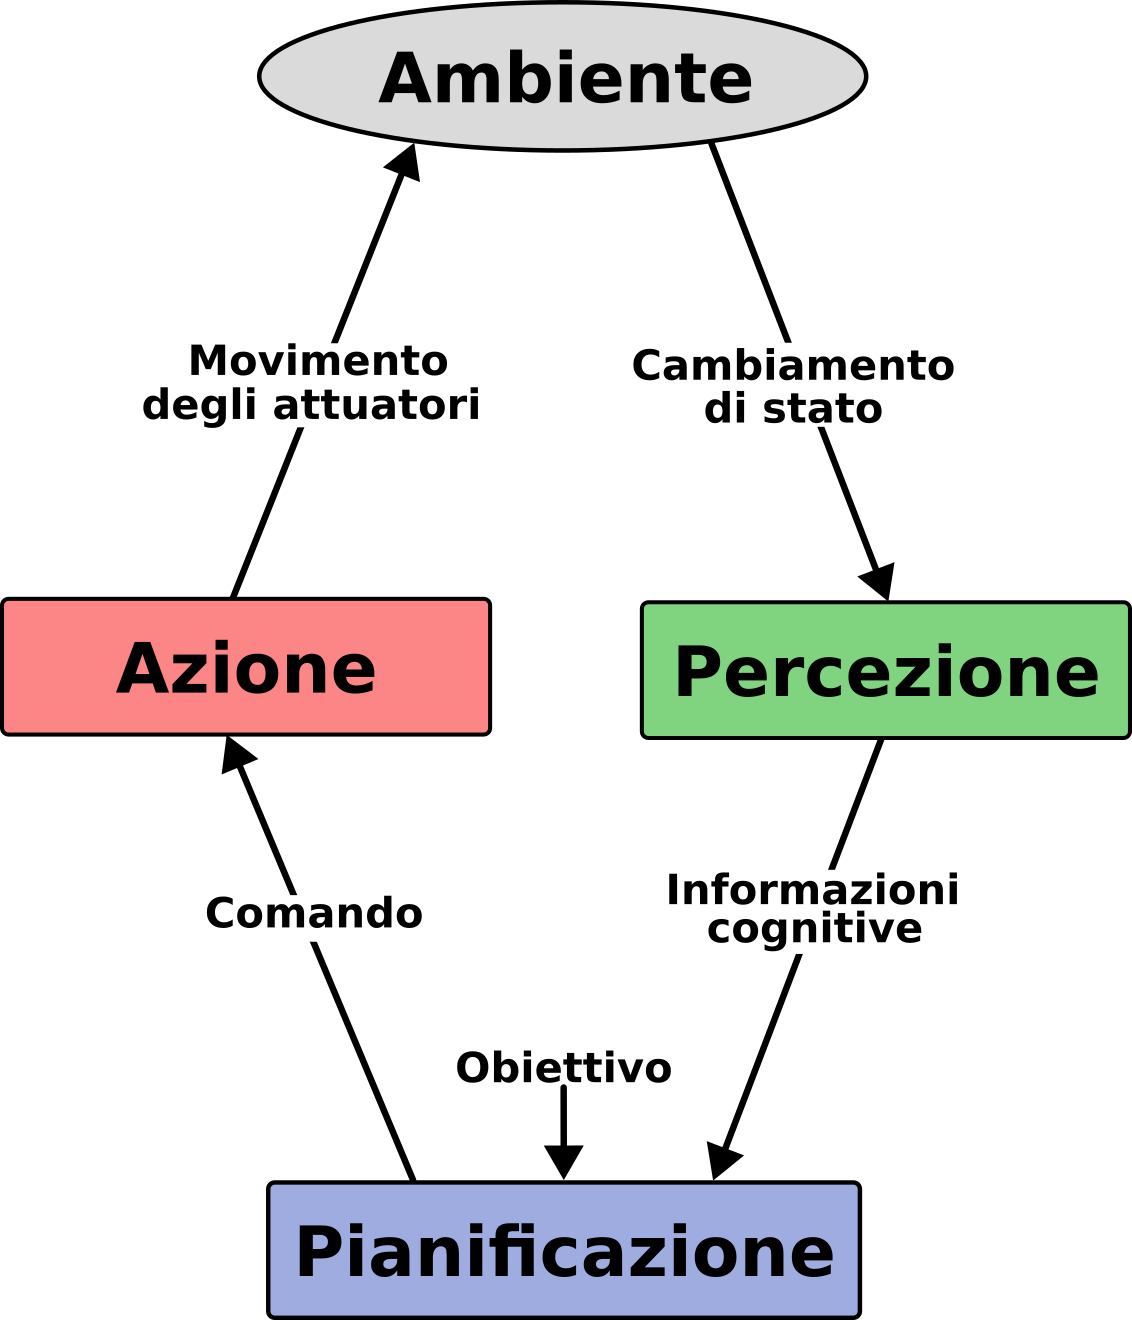
\includegraphics{architecture.png}
\column{0.01\textwidth}
\column{0.49\textwidth}
\centering
Entry point del modulo software \\
\begin{lstlisting}
function start
	error = norm([xr,yr]-G);
	while(error > 0.1)
		%Detected obstacle 
		dObstacle = sense.scan();
		%New directive
		state.decision(dObstacle);
		%Commands to the actuators 
		newPose = act.move(tspan);
		%Refreshing the error
		error = norm([xr,yr]-G);
	end
end
\end{lstlisting}
\end{columns}
\end{frame}


\begin{frame}{Modulo di pianificazione}
\centering
%{\Large \textbf{Modulo di pianificazione}}
\begin{figure}
%\vspace{10mm}
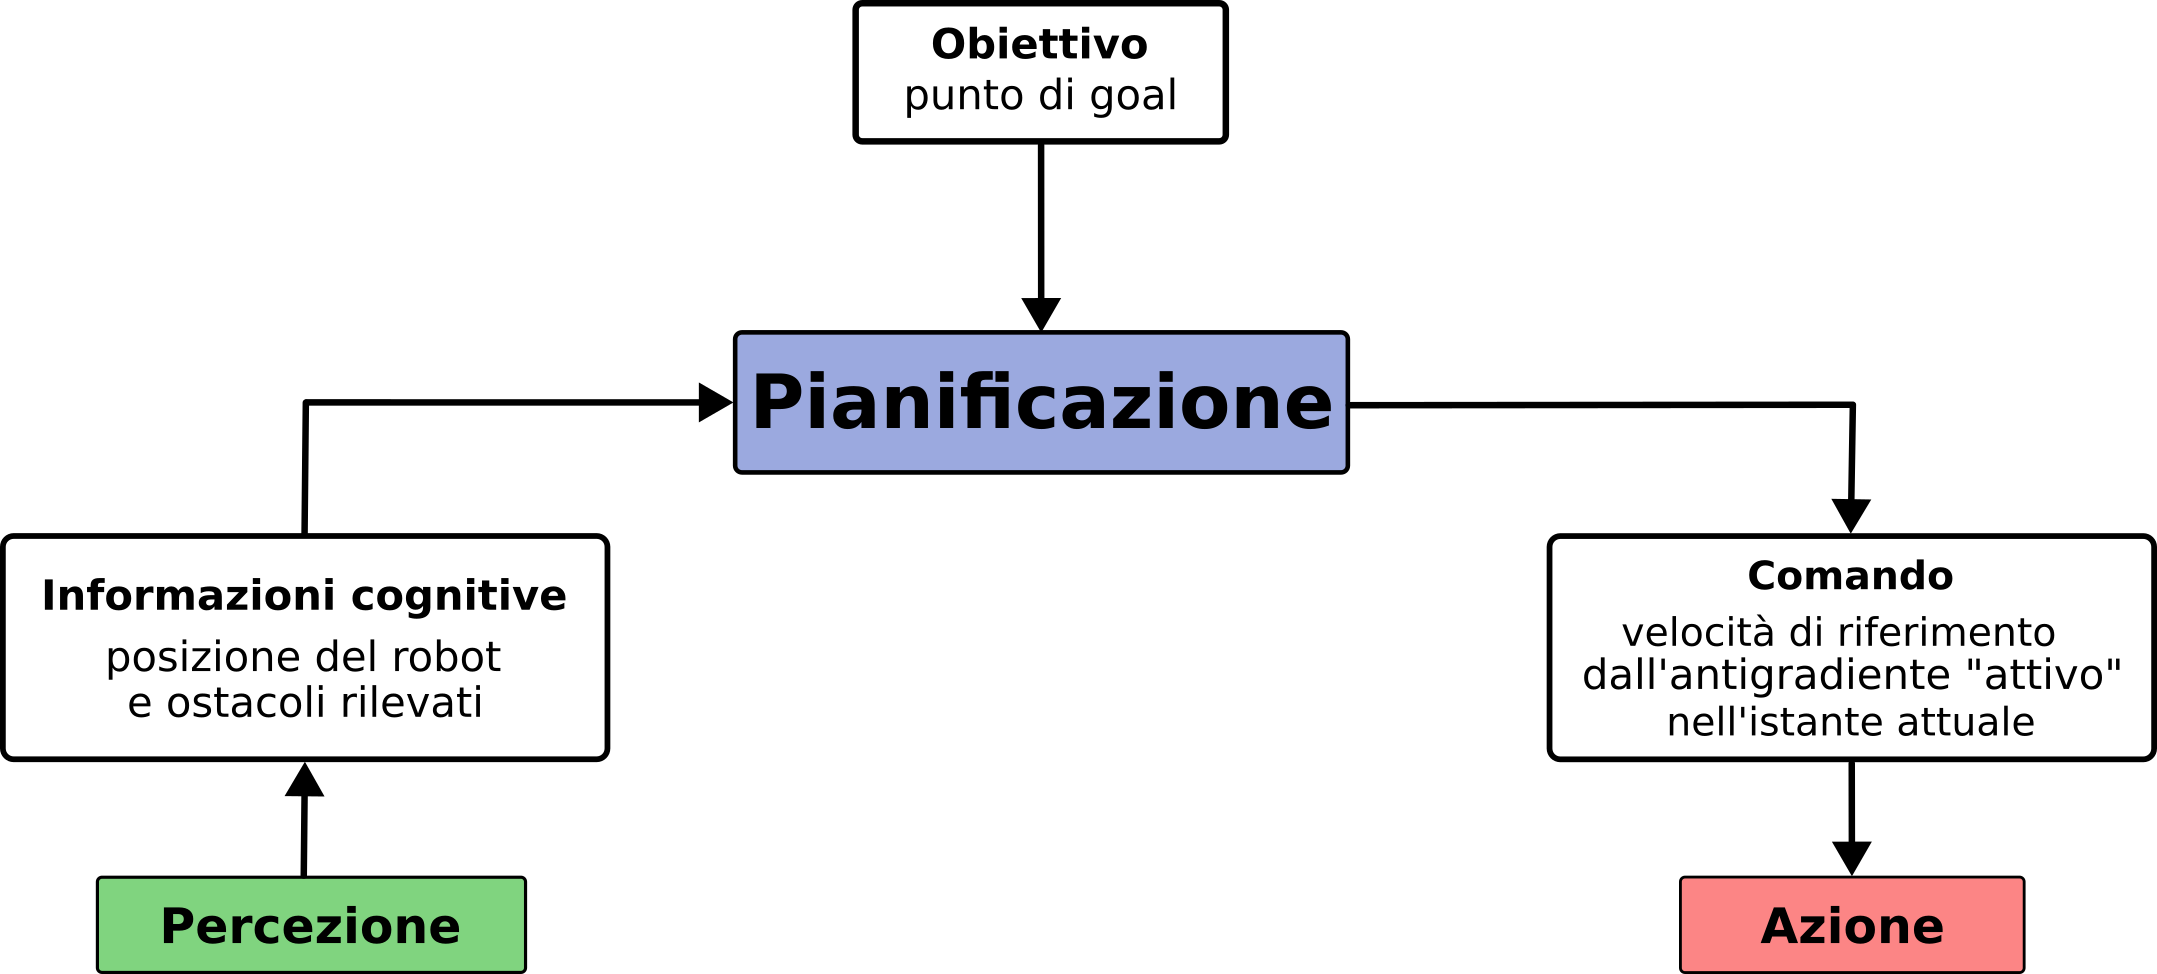
\includegraphics[scale=1]{pianificazione.png}
\end{figure}
\end{frame}

%30 secondi
\begin{frame}{Modulo di pianificazione}
\framesubtitle{Design pattern State}
\centering
\hspace{2cm}
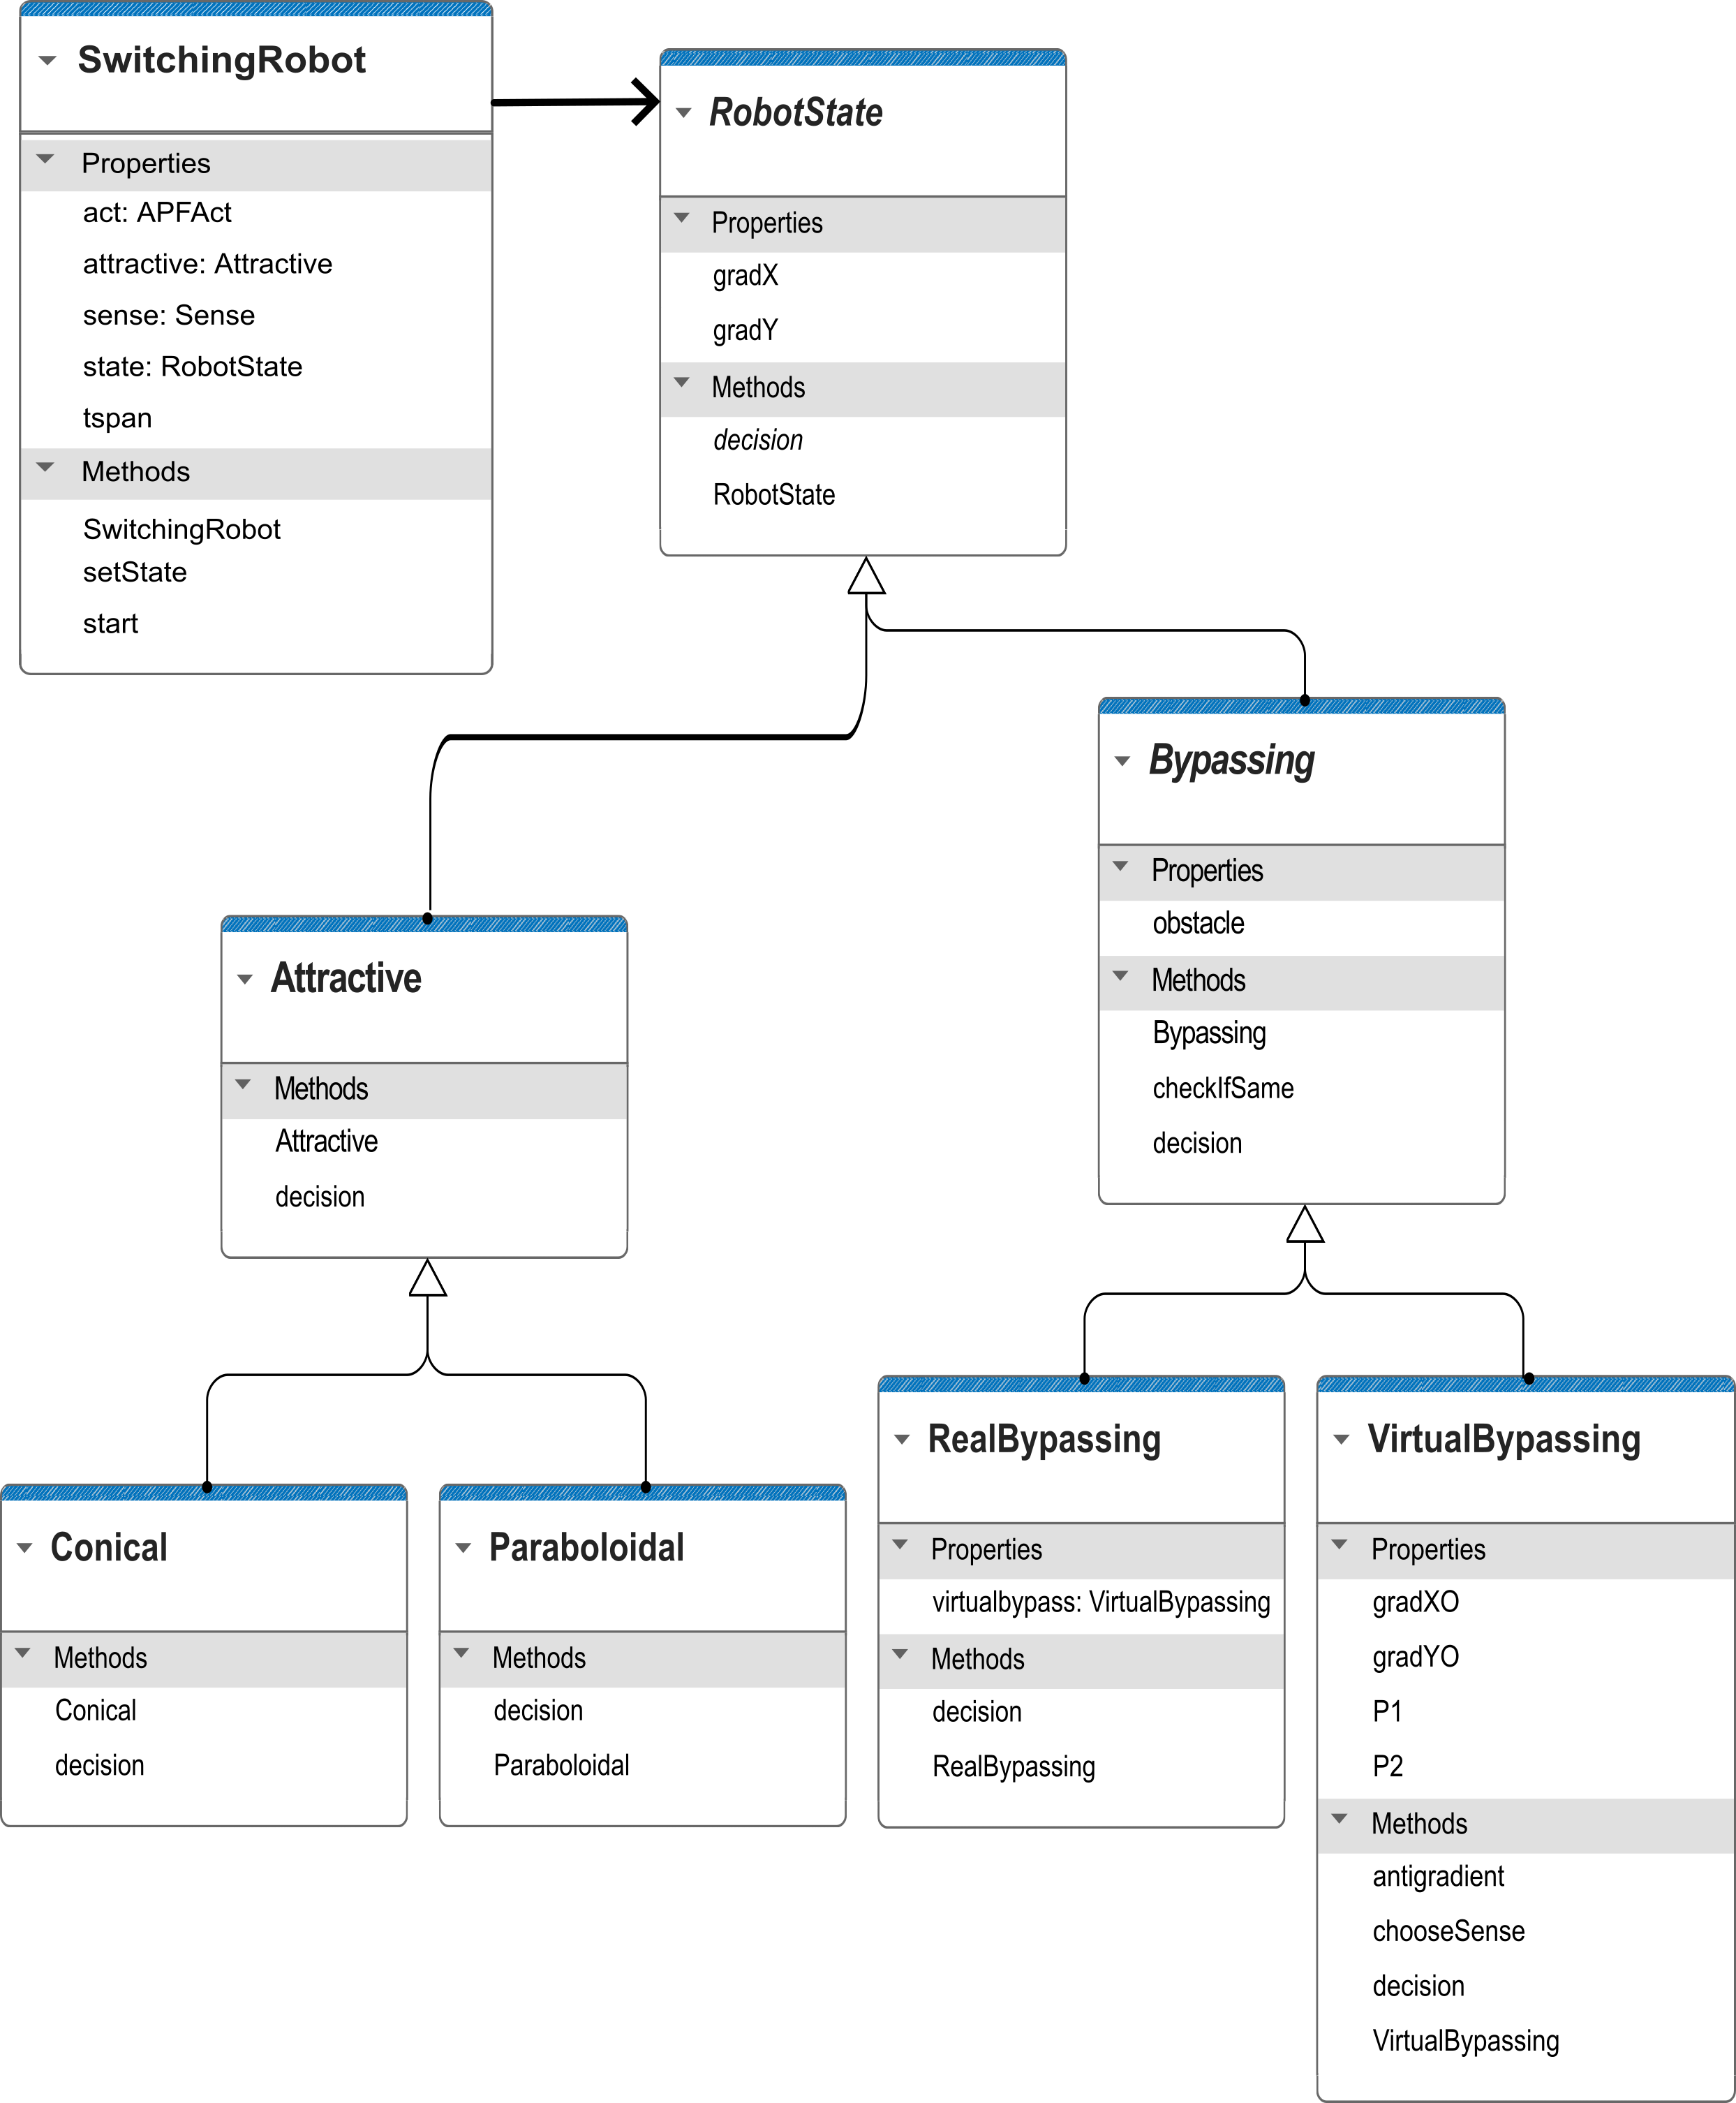
\includegraphics[scale=1.07]{pianificazioneclass.png}
\end{frame}

%1 minuto
\begin{frame}{Modulo di pianificazione}
\framesubtitle{Switching : scelta del verso di bypassing}
\begin{columns}
\column{0.45\textwidth}
\centering
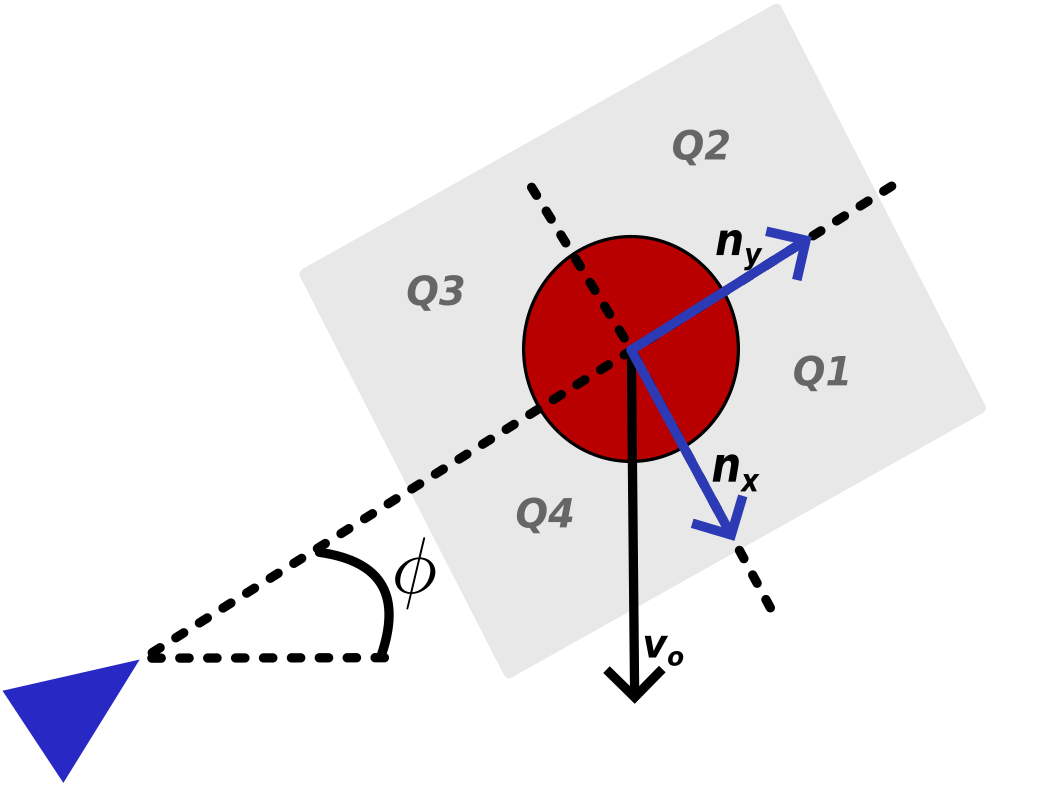
\includegraphics{sceltaverso.png}
\column{0.1\textwidth}
\centering
$\rightarrow$
\column{0.45\textwidth}
\centering
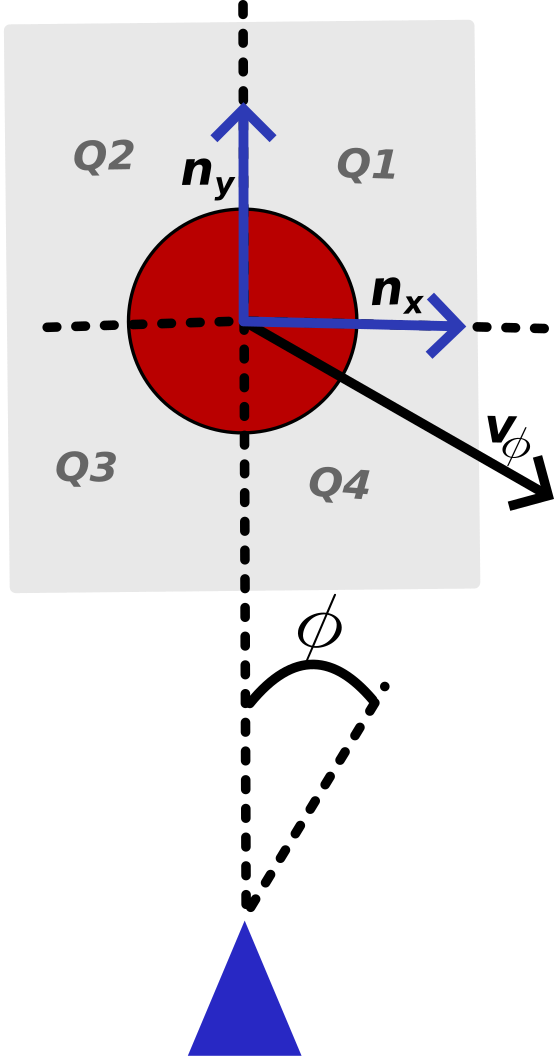
\includegraphics{sceltaversogirato.png}
\end{columns}
\centering
\[
\begin{cases}
\cos{v_{\phi}} \geq 0 \Rightarrow orario \\
\cos{v_{\phi}} < 0 \Rightarrow antiorario
\end{cases}
\]
\end{frame}

%1 minuto
\begin{frame}{Modulo di pianificazione}
\framesubtitle{Switching: assenza di discontinuità}
\begin{columns}
\column{0.5\textwidth}
\centering
\hspace*{-5mm}
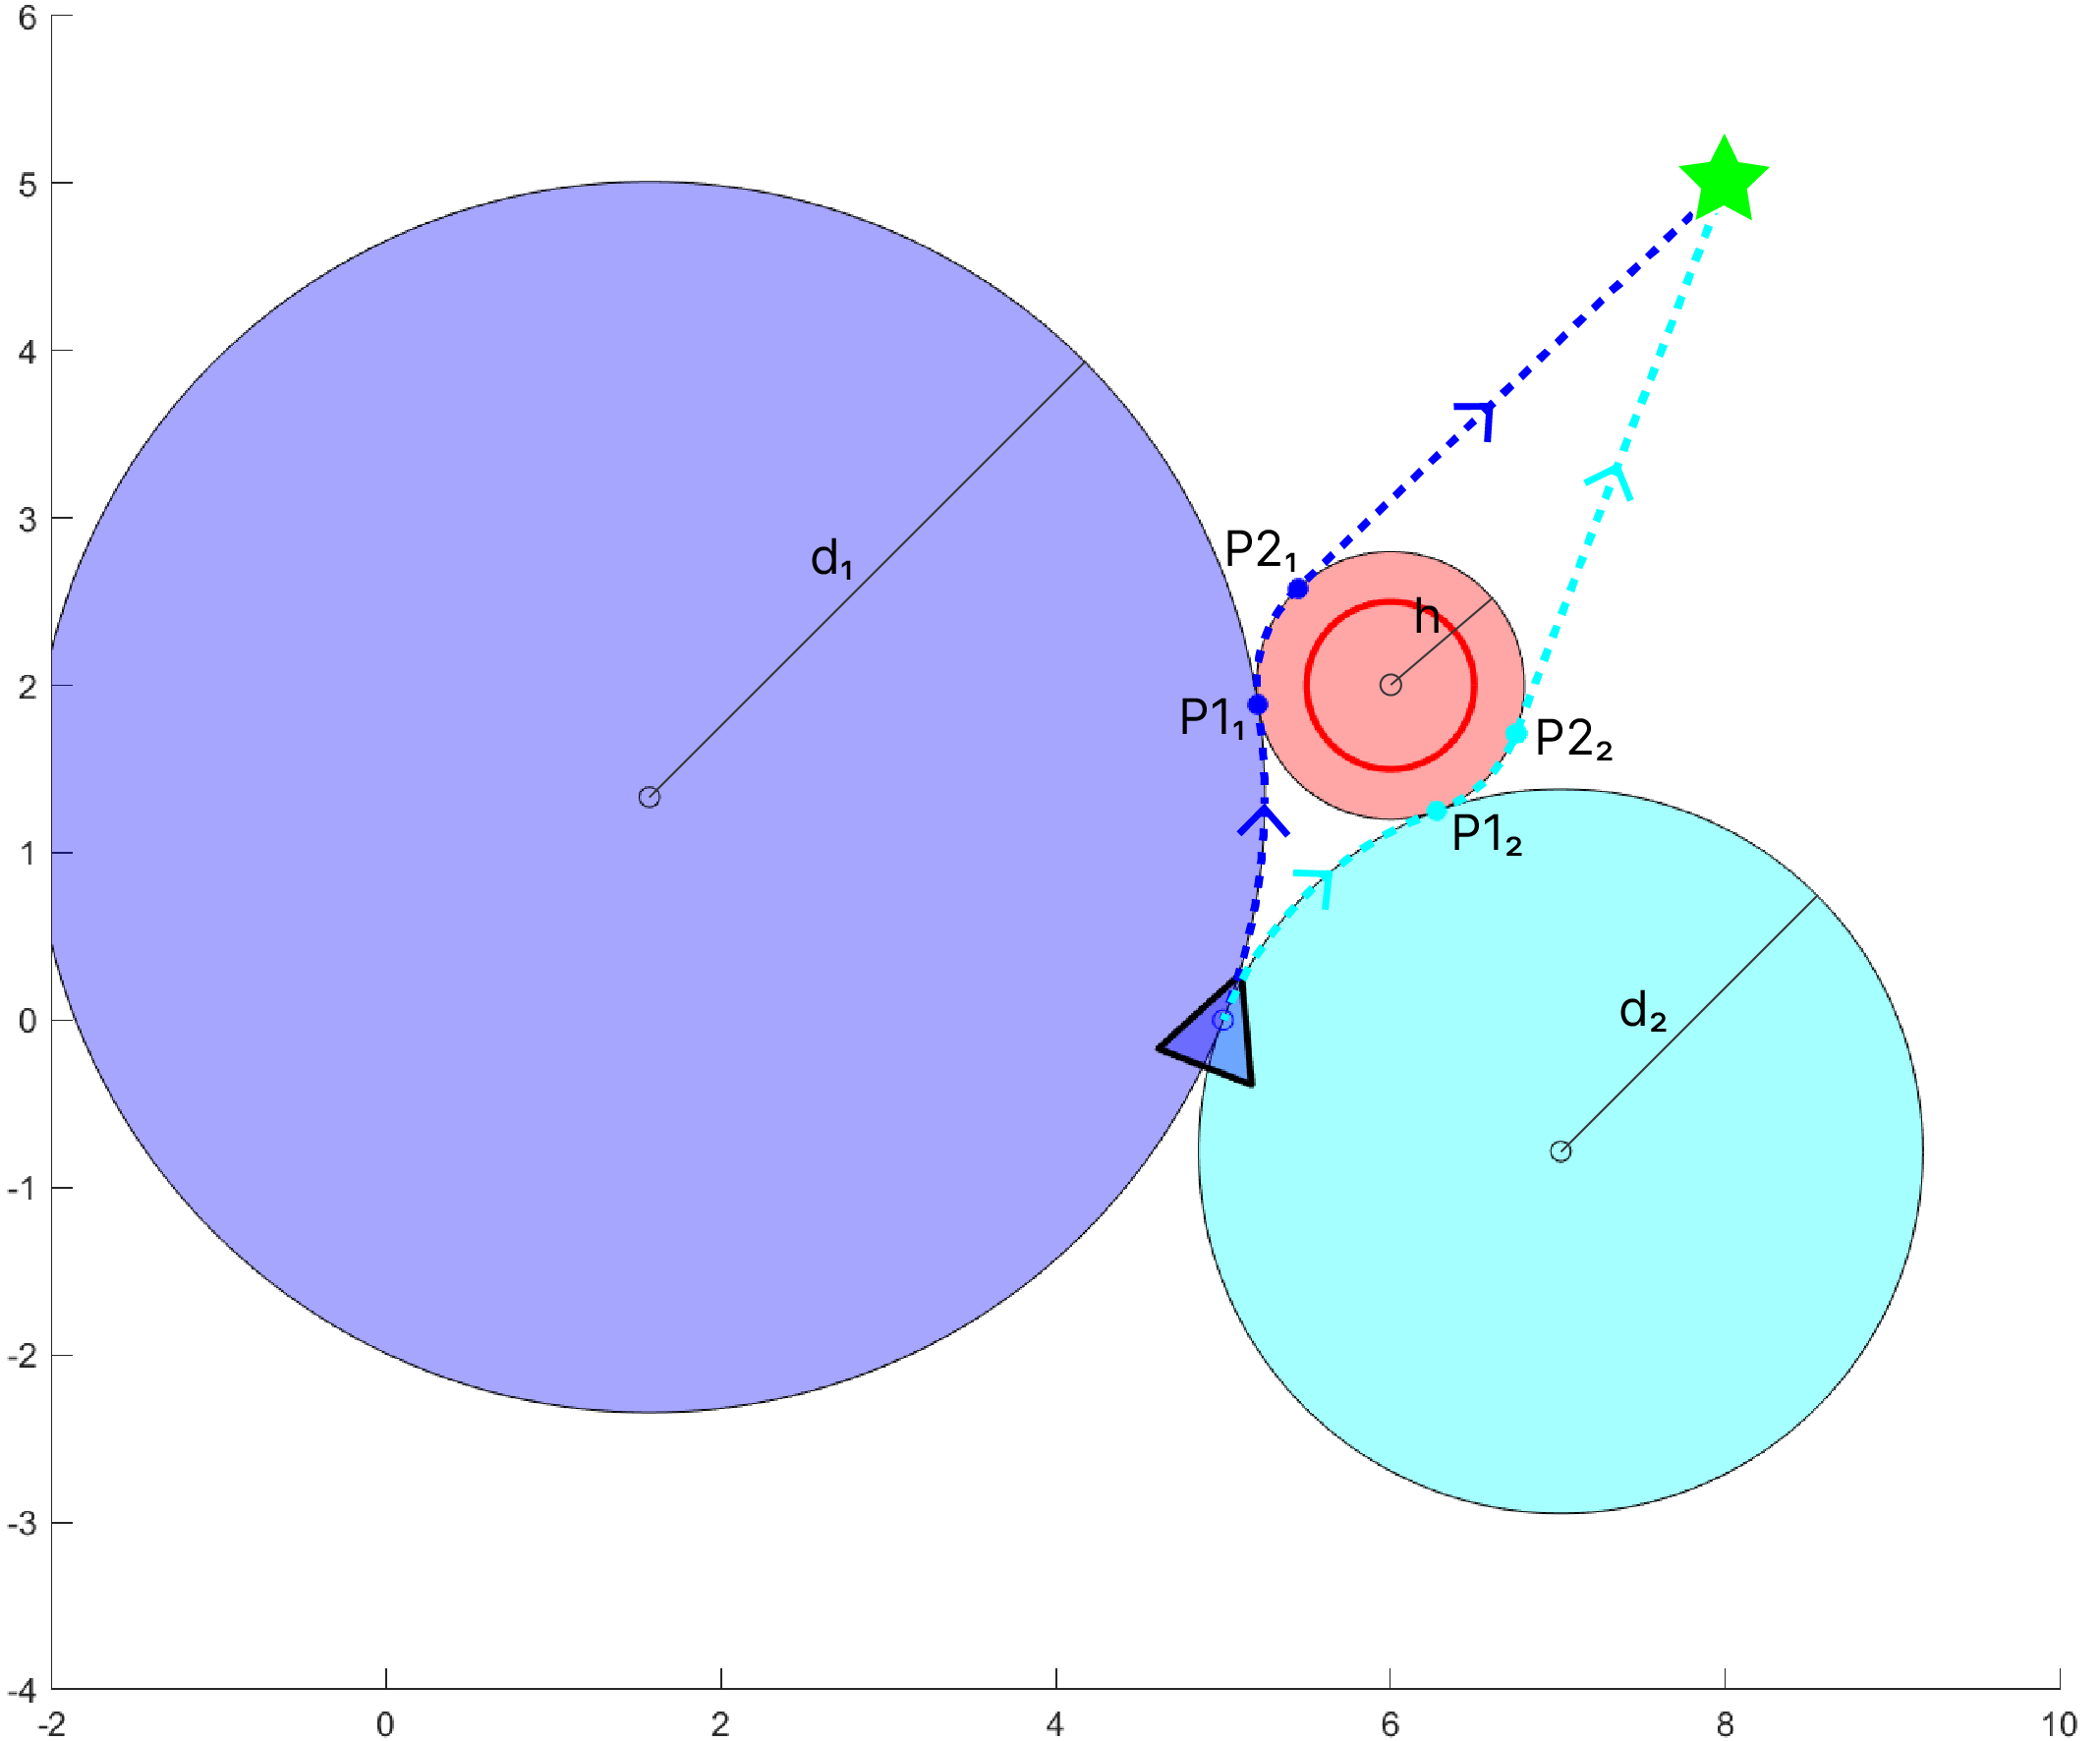
\includegraphics[width=1.1\textwidth]{circonferenze.png}
\column{0.5\textwidth}
\centering
\begin{figure}
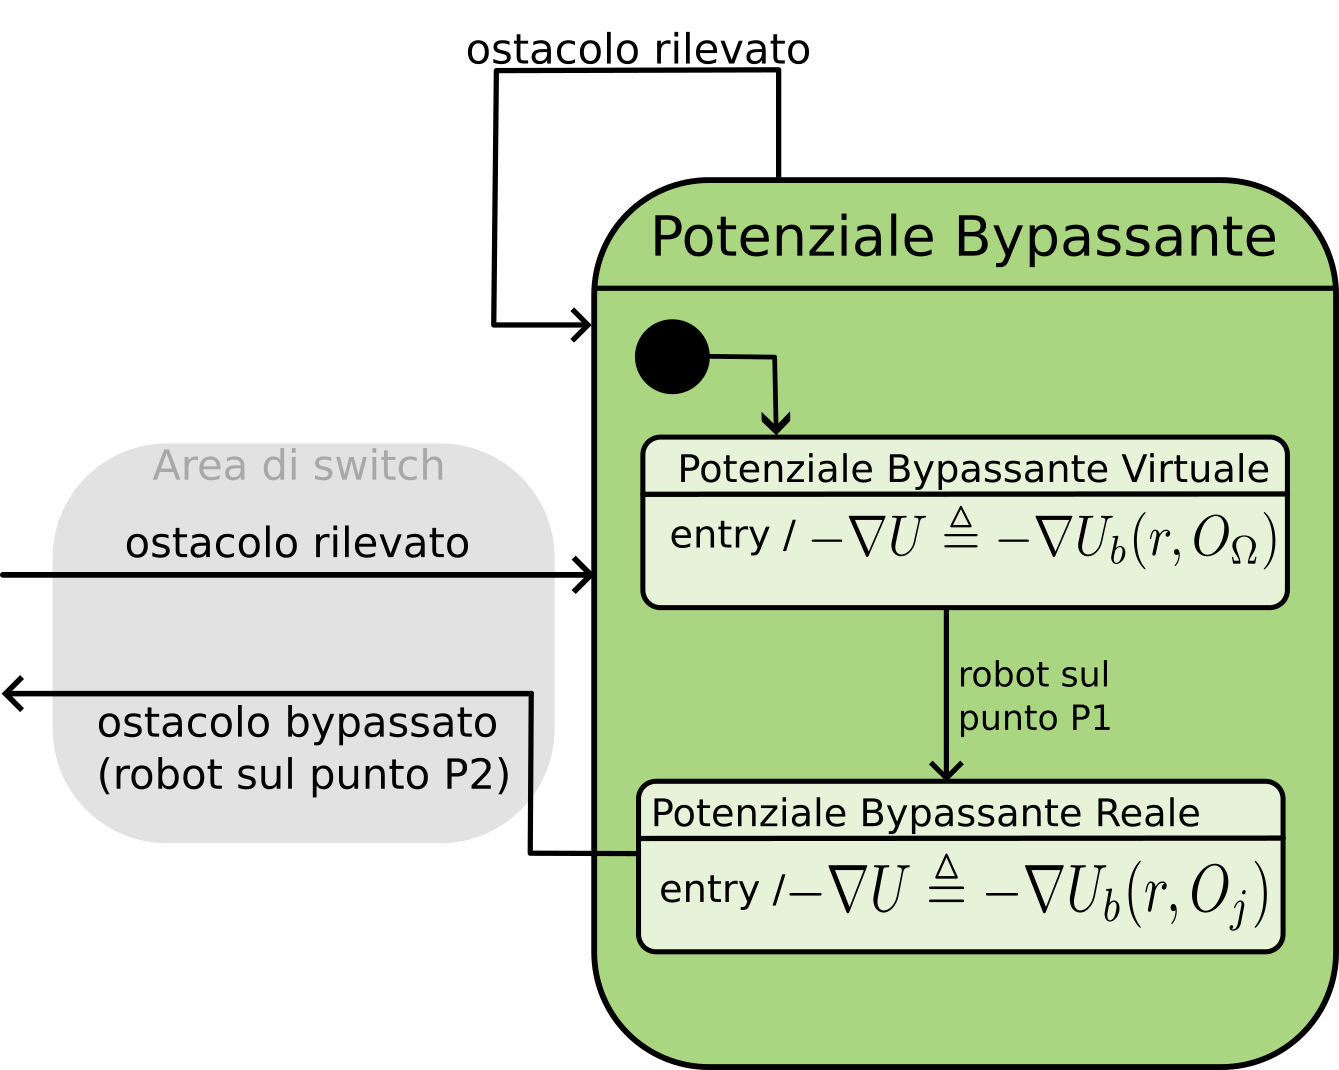
\includegraphics[width=0.8\textwidth]{statechartbypassante.png}
\end{figure}
\vspace{10mm}
\begin{itemize}
\item Ostacolo fermato in $\tau$
\item Ausilio di ostacolo virtuale
\item Condizioni di tangenza sulle curve di livello del potenziale bypassante
\end{itemize}
\end{columns}
\end{frame}

%20 secondi
\begin{frame}{Modulo di azione}
\centering
%{\Large \textbf{Modulo di azione}}
\begin{figure}
%\vspace{10mm}
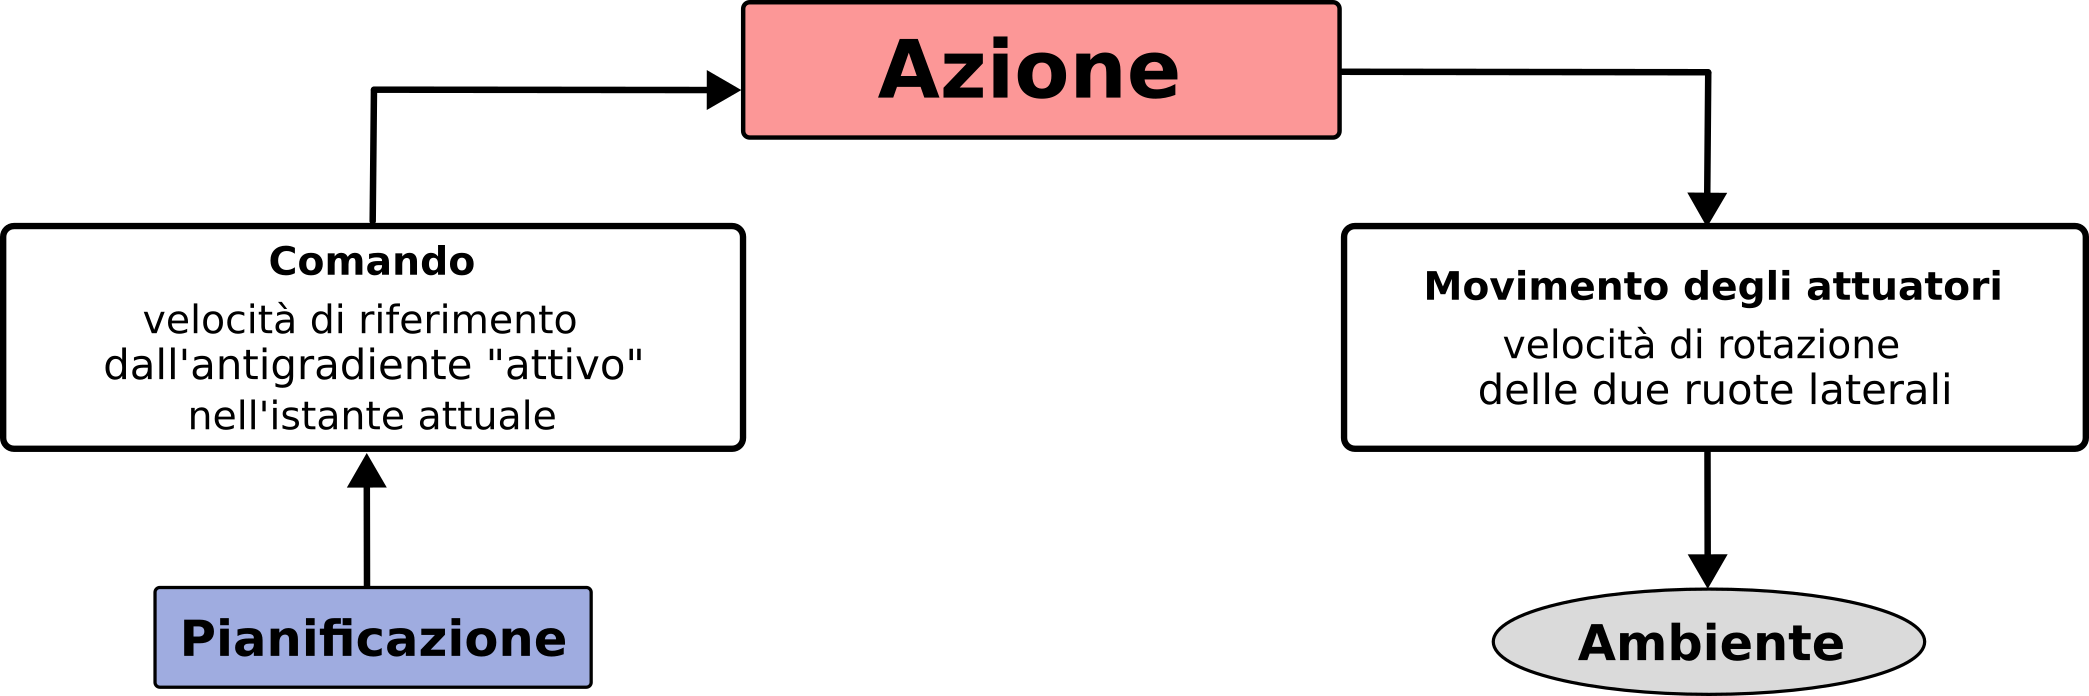
\includegraphics{azione.png}
\end{figure}
\end{frame}

%30 secondi
\begin{frame}{Modulo di azione}
\framesubtitle{Legge di controllo}
\begin{itemize}
\item Obiettivo: ottenere dei comandi di velocità 
\item Nello specifico $v(t)$ velocità lineare e $\omega(t)$ velocità angolare
\item Velocità di riferimento é $v_{\nabla}(t) \triangleq -\nabla U(r,G)$
\end{itemize}
\vspace{2mm}
Imponendo
\begin{equation}
v(t) = M_v \cos(\theta_{\nabla}(t) - \theta_r(t))
\end{equation}
\begin{equation}
\omega(t) = K_{\omega}(\theta_{\nabla}(t) - \theta_r(t))
\end{equation}
dove \(M_v=\begin{Vmatrix}v_{\nabla}(t)\end{Vmatrix}\), \(\theta_{\nabla}=\angle v_{\nabla}(t)\) e \\
\(K_{\omega}(t)= \begin{cases}
\frac{\dot{\theta}_{\nabla}(t) + K_c|\theta_{\nabla}(t)-\theta_r(t)|^{\nu} \cdot sign(\theta_{\nabla}(t) - \theta_r(t))}{\theta_{\nabla}(t) - \theta_r(t)} \ &|\theta_{\nabla}(t)-\theta_r(t)| \geq \xi \\
0 \ &altrimenti
\end{cases}\)
\end{frame}

\renewcommand{\arraystretch}{1.5}
%40 secondi
\begin{frame}{Modulo di azione}
\framesubtitle{Modello cinematico}
\begin{columns}
\column{0.45\textwidth}
\centering
$
\begin{cases}
\dot{x}(t) = v(t)\cos(\theta(t)) \\
\dot{y}(t) = v(t)\sin(\theta(t)) \\
\dot{\theta}(t) = \omega(t)
\end{cases}
$
\column{0.02\textwidth}
\centering
$\Rightarrow$
\column{0.53\textwidth}
\centering
$
\begin{cases}
\dot{x}(t) = \frac{R}{2} \left( \omega_R(t)+\omega_L(t) \right) \cos(\theta(t)) \\
\dot{y}(t) = \frac{R}{2} \left( \omega_R(t)+\omega_L(t) \right)\sin(\theta(t)) \\
\dot{\theta}(t) = \frac{R}{L} \left( \omega_R(t)-\omega_L(t) \right)
\end{cases}
$
\end{columns}
\vspace{5mm}
\begin{columns}
\column{0.5\textwidth}
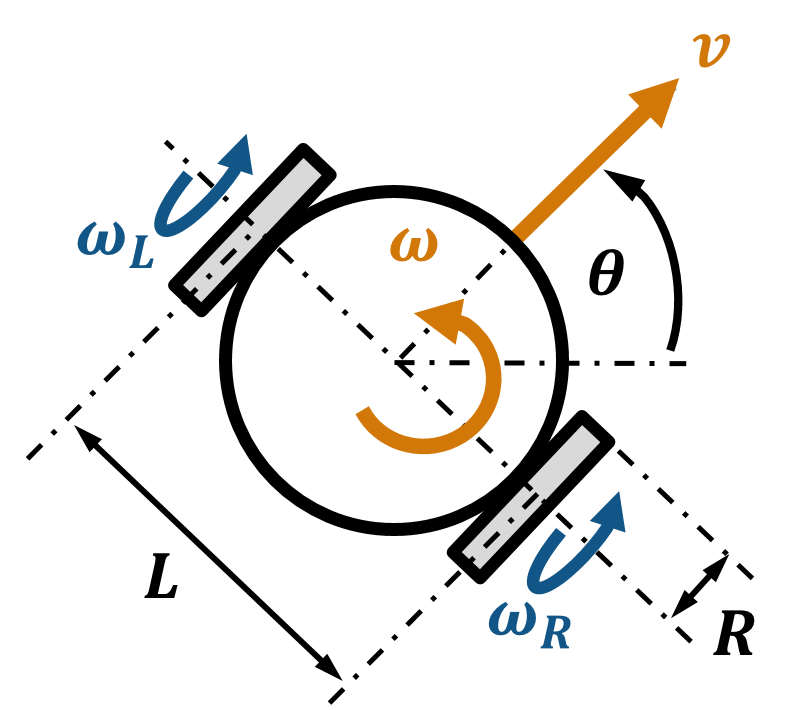
\includegraphics[width=\textwidth]{DD.png}
\column{0.5\textwidth}
\centering
Dettaglio: velocità delle ruote \\
$
{\begin{bmatrix}
\omega_R(t) \\
\omega_L(t)
\end{bmatrix} =
\begin{bmatrix*}[r]
\frac{R}{2} & \frac{R}{2} \\
\frac{R}{L} & -\frac{R}{L}
\end{bmatrix*}^{-1}
\begin{bmatrix}
v(t) \\
\omega(t)
\end{bmatrix}}$
\end{columns}
\end{frame}

%20 secondi
\begin{frame}{Modulo di percezione}
\centering
%{\Large \textbf{Modulo di percezione}}
\begin{figure}
%\vspace{10mm}
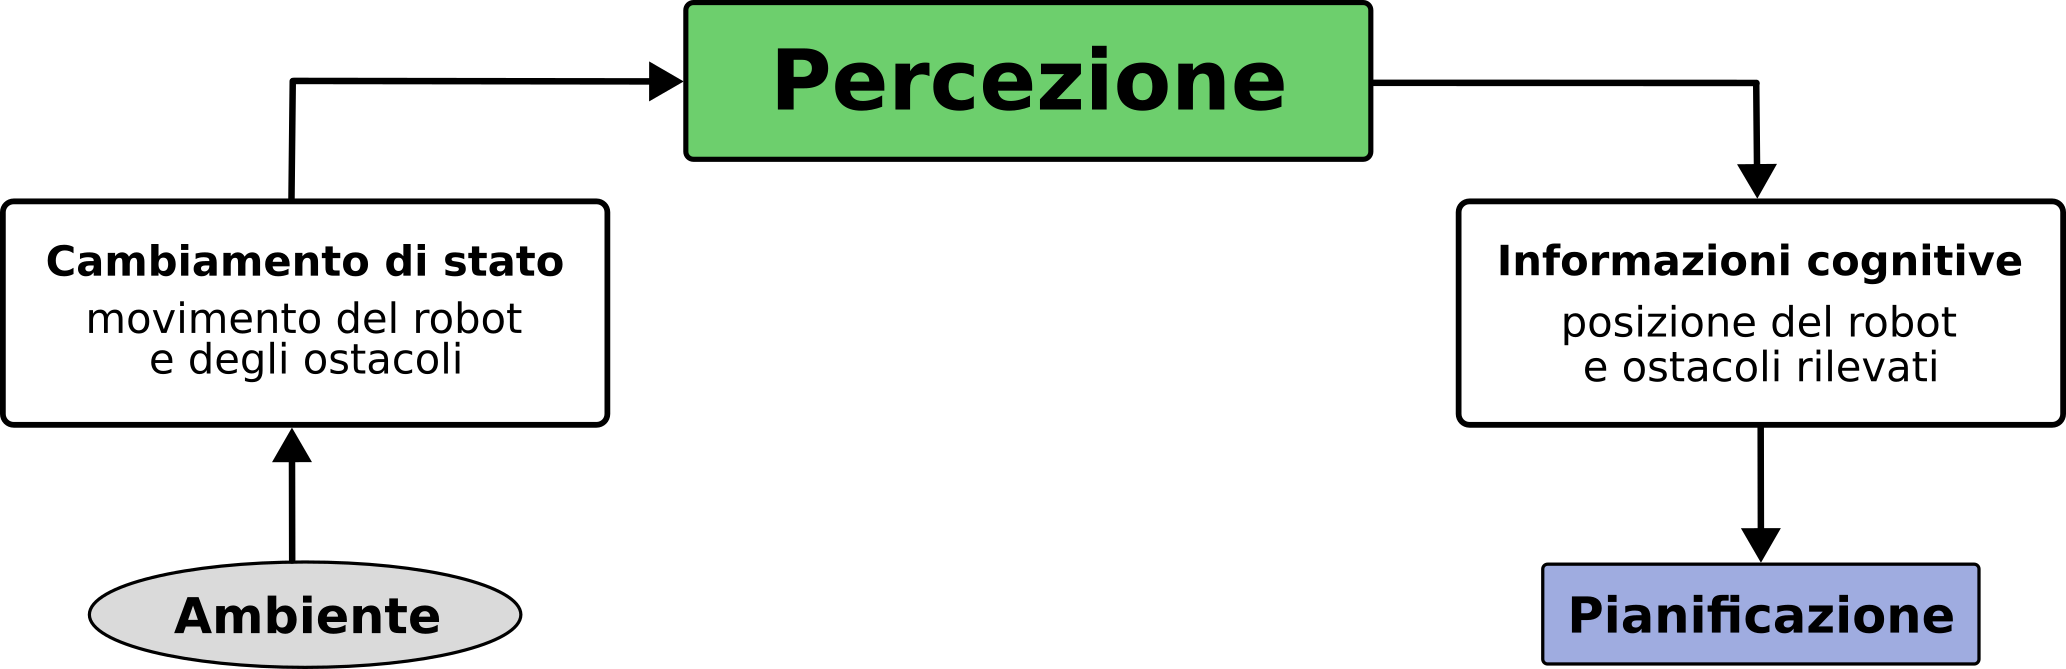
\includegraphics{percezione.png}
\end{figure}
\end{frame}

%1 minuto
\begin{frame}{Modulo di percezione}
\begin{columns}
\column{0.65\textwidth}
	\centering
	\begin{itemize}
	\item Raggio di visione $R_v$
	\item Tubo verso il goal di larghezza $R_T$
	\item Localizzazione sul centro dell'ostacolo
	\end{itemize}
	\[\Downarrow\]
L'ostacolo da bypassare é quello, se c'è, che si trova nel tubo ad una distanza dal robot minore di tutti gli altri ostacoli nel tubo
\column{0.35\textwidth}
	\centering
	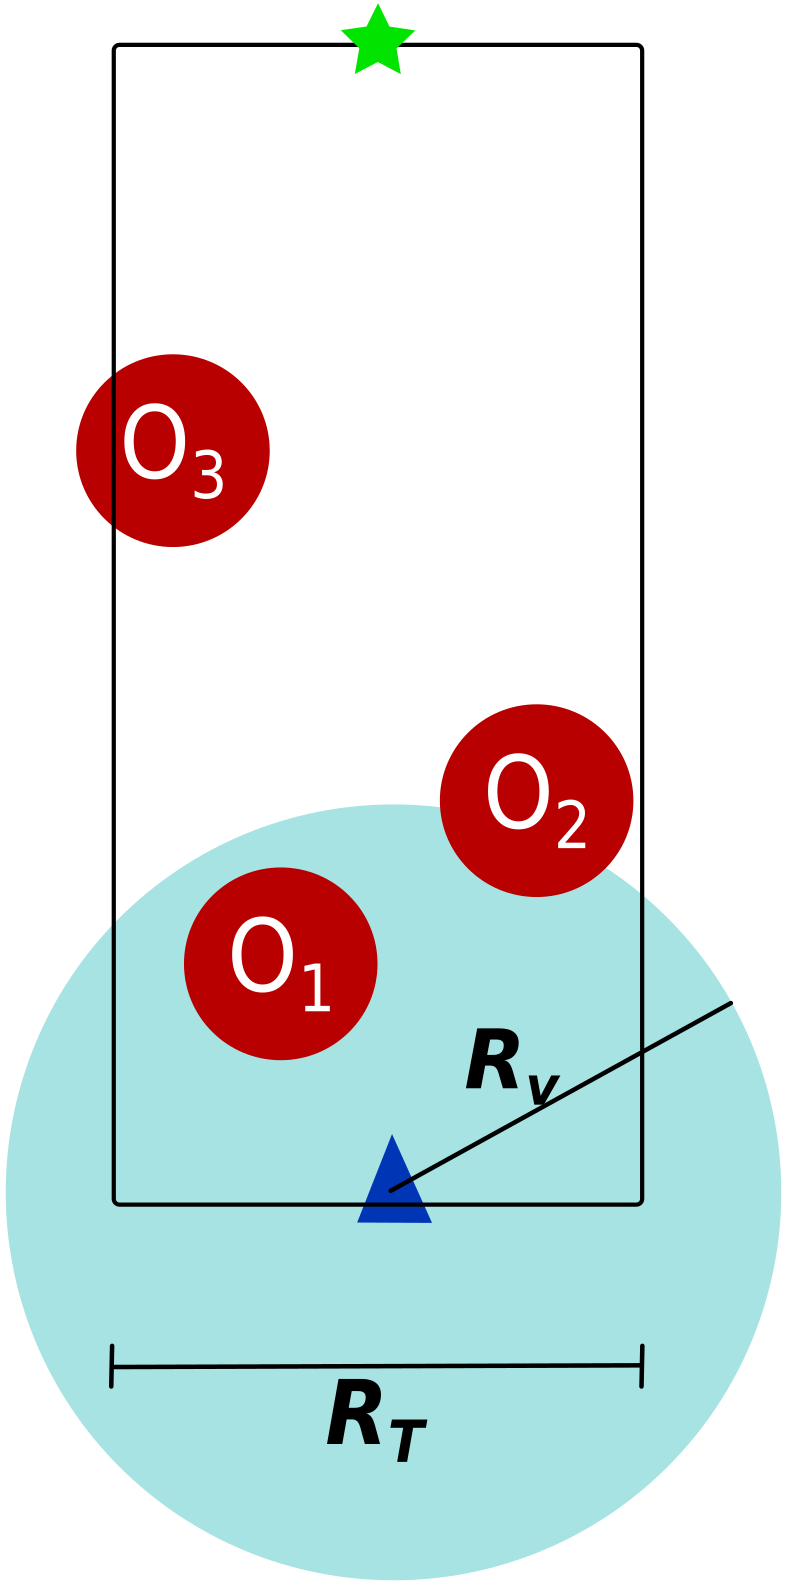
\includegraphics[scale=1]{tubo.png}
\end{columns}
\end{frame}

%30 secondi
\begin{frame}{Risultati}
\framesubtitle{Tre ostacoli in movimento}
\centering
\graphicspath{ {../simulazioni/treostacoli1} }
\animategraphics[loop,width=8cm]{20}{snap}{1}{253}
\end{frame}

%30 secondi
\begin{frame}{Risultati}
\framesubtitle{Cinque ostacoli in movimento}
\centering
\graphicspath{ {../simulazioni/treostacoli1} }
\animategraphics[loop,width=8cm]{20}{snap}{1}{253}
\end{frame}

%30 secondi
\begin{frame}{Risultati}
\framesubtitle{Tredici ostacoli fissi}
\centering
\graphicspath{ {../simulazioni/moltiostacoli} }
\animategraphics[loop,width=8cm]{10}{snap}{1}{322}
\end{frame}

%30 secondi
\begin{frame}{Risultati}
\framesubtitle{Rischio minimo locale}
\centering
\graphicspath{ {../simulazioni/treostacoli1} }
\animategraphics[loop,width=8cm]{20}{snap}{1}{253}
\end{frame}

\end{document}